\section{Factorial Treatment Structure}

Often treatments are combinations of the levels of two or more factors, this is called \textbf{factorial treatment structure}. If we observe all possible combinations, we call them \textbf{crossed}.

\begin{lstlisting}
xtabs(~ factor1 + factor2, data = d)
\end{lstlisting}

This typically leads to questions about the interaction of the different factors (or if the interact at all).


\subsection{Two-Way ANOVA Model}

We assume a setup with a factor $A$ with $a$ levels, a factor $B$ with $b$ levels and $n$ replicates for every combination (a \textbf{balanced} design). We denote by $y_{ijk}$ the $k$th observation of the response of the treatment formed by the $i$th level of factor $A$ and the $j$th level of factor $B$. Instead of setting up a model for each combination, we incorporate the factorial treatment structure directly into the \textbf{two-way ANOVA model with interaction}:
$$Y_{ijk} = \mu + \alpha_i + \beta_j + (\alpha \beta)_{ij} + \epsilon_{ijk}$$

Hereby $\alpha, \beta$ are the main effect of factor $A, B$ and $(\alpha \beta)$ is the interaction effect. A model without interaction term is additive, meaning that the effect of $A$ does not depend on the effect of $B$.\medskip

As usual, we'll have to use side constraints for the parameters (we will use the sum-to-zero constraint). For the main effects:
$$\sum_{i=1}^a \alpha_i = 0 \qquad \sum_{j=1}^b \beta_j = 0 $$

Hence they both have $a-1$ / $b-1$ degrees of freedom. For the interaction effect we need to make sure that it contains nothing which is specific to one factor:
$$\sum_{i=1}^a (\alpha \beta)_{ij} = 0 \qquad \sum_{j=1}^b (\alpha \beta)_{ij} = 0$$

Therefore the interaction term has a degree of freedom of $(a-1)(b-1)$.

\subsubsection{Parameter Estimation}

We estimate parameters using least squares and the sum-to-zero side constraints. We get the following parameter estimates:
\begin{align*}
	\hat \mu &= \bar y_{...} \\
	\hat \alpha_i &= \bar y_{i..} - \bar y_{...} \\
	\hat \beta_j &= \bar y_{.j.} - \bar y_{...} \\
	\widehat {(\alpha \beta)}_{ij} &= \bar y_{ij.} - \hat \mu - \hat \alpha_i - \hat \beta_j
\end{align*}

We end up with the mean of the observations in the corresponding cell as the expected value of the response $Y_{ijk}$.

\begin{lstlisting}
fit <- aov(y ~ a * b, data = d) 
## alternatively: aov(y ~ a + b + a:b, data = d)
\end{lstlisting}

\subsubsection{Tests}

The total sum of squares $SS_T$ can be partitioned into different sources.
$$SS_T = SS_A + SS_B + SS_{AB} + SS_E$$

\begin{center}
	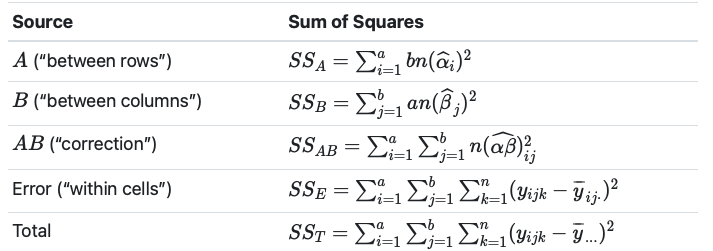
\includegraphics[width=\linewidth]{ss-two-way-ANOVA.png}
\end{center}

We can again construct an ANOVA table:
\begin{center}
	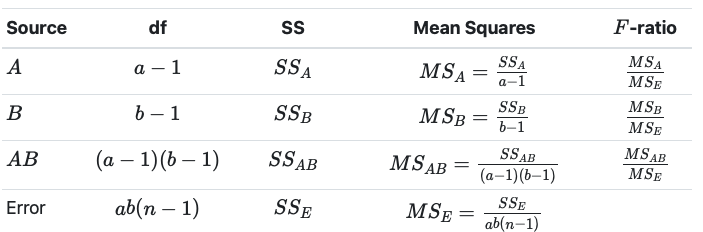
\includegraphics[width=\linewidth]{two-way-ANOVA.png}
\end{center}
In general, the degree of freedom of the error term is given by $N - (\text{DF } A) - (\text{DF } B) - (\text{DF } AB) - 1$. \medskip

We now want to construct global tests for the main effects and the interaction effect: \medskip

\textbf{Interaction Effect:} The null hypothesis that there is no interaction effect can be seen as: "The effect of factor $A$ does not depend on the level of factor $B$ or the other way around". $H_0: \forall ij. \; (\alpha \beta)_{ij} = 0$. Under $H_0$ it holds that:
$$\frac{MS_{AB}}{MS_E} \sim F_{(a-1)(b-1),ab(n-1)}$$

\textbf{Main Effect of $A$:} $H_0: \forall i. \; \alpha_i = 0$. Under $H_0$ it holds that:
$$\frac{MS_{A}}{MS_E} \sim F_{(a-1), ab(n-1)}$$
 
\textbf{Main Effect of $B$:} $H_0: \forall j. \; \beta_j = 0$. Under $H_0$ it holds that:
$$\frac{MS_{B}}{MS_E} \sim F_{(b-1), ab(n-1)}$$

In R, we get the ANOVA table and the corresponding p-values again with the \textit{summary} function. We first check whether we need the interaction term or not. If there is no evidence of interaction, we continue with the inspection of the main effects. The degree of freedom of the interaction form is the product of factors involved, e.g. $(a-1)(b-1)$.

\subsubsection{Individual Analysis}

If we have two factors $A, B$ then instead of a full model, we might want to choose one model per individual level of $A$ (e.g. due to some interaction). This can be improved by reusing the $MS_E$ with the degree of freedom of the full model. This leads to a better power because the quantiles of the $F$-distribution will be smaller. Similar for contrasts we can use $\sigma^2$ estimates given by the $MS_E$ of the full model. This is especially useful if the degree of freedom of the error term is small ($< 10$).

\subsubsection{Single Observations per Cell}

If we only have a single observation in each "cell", we cannot do statistical inference anymore with a model including the interaction. The reason is that we have no idea of the experimental error. However, we can still fit a main effects only model. If the data generating mechanism actually contains an interaction, we are fitting a wrong model. The consequence is that the estimate of the error variance will be biased (upward). Hence, the corresponding tests will be too conservative, meaning p-values will be too large and confidence intervals too wide. This is not a problem as the type I error rate is still controlled; we “just” lose power. \medskip

Quite often, we can get rid of interactions if we look at the problem on a different scale, i.e. if we transform the response appropriately. A famous example is the logarithm. Effects that are multiplicative on the original scale become additive on the log-scale, i.e. no interaction is needed on the log-scale.\medskip

If we have no replicates and more than two factors we often remove higher-order interaction terms (goes into error term).

\subsubsection{Tukey One DF Interaction}

The idea is to use only one additional term for the interaction. For a two-factor model this looks like the following:
$$Y_{ij} = \mu + \alpha_i + \beta_j + \lambda \alpha_i \beta_j + \epsilon_{ij}$$

$\lambda$ is the new term and $\alpha_i \beta_j$ is the product of the main effects.

\subsubsection{Checking Model Assumptions}

As before, we use the QQ-plot and the Tukey-Anscombe plot to check the model assumptions.

\subsubsection{Unbalanced Data}

We started with the very strong assumption that our data is balanced, i.e., we have the same number of replicates. This assumption made our life "easy" in the sense that we could uniquely decompose total variability into different sources and we could estimate the parameters of the coefficients of a factor by ignoring the other factors. \textbf{In practice, data is typically not balanced and we cannot decompose the variability}. This problem can be solved by using a model comparison approach. \medskip

We use the following notation: $SS( B | 1, A)$ denotes the \textbf{reduction in residual sum of squares} when comparing the model $(1, A, B) = y \sim A + B$ with $(1, A) = y \sim A$. The 1 denotes the overall mean $\mu$. Interpretation of the corresponding test is as follows: "Do we need factor B in the model if we already have factor A, or after having controlled for factor A?". \medskip

There are three different ways of model comparison approaches:
\begin{itemize}
	\item Type 1 (sequential): $SS(A | 1) \to SS(B | 1, A) \to SS(AB | 1, A, B)$
	\item Type 2 (hierarchical): $SS(A | 1, B) \to SS(B | 1, A) \to SS(AB | 1, A, B)$
	\item Type 3 (fully adjusted): $SS(A | 1, B, AB) \to SS(B | 1, A, AB) \to SS(AB | 1, A, B)$
\end{itemize}

The tests are the same for the interaction term. For the $B$ factor type 1 and type 2 are the same. \medskip

Type 1 is what we will typically get with \textit{summary} in R. Hence we get different results whether we write $y \sim A * B$ or $y \sim B * A$. For type 2 we can either use the function \textit{Anova} in the package \textit{car} or we could compare the appropriate models with the function \textit{anova} ourselves. For type 3 we can use the command \textit{drop1}; we have to be careful that we set the contrast option to \textit{contr.sum} in this special situation for technical reasons, see also the warning in the help file of the function \textit{Anova} of package \textit{car}.

\begin{lstlisting}
## Type II sum of squares (Type III is similar)
library(car)
Anova(fit, type = "II", data = d)	
\end{lstlisting}

Typically, we take $MS_E$ from the full model (including all terms) as the estimate for the error variance to construct the corresponding $F$-tests.
